\documentclass[a4paper,norsk]{article}
\usepackage{graphicx}
\usepackage{sidecap}
\usepackage{wrapfig}
\usepackage{preamble}


\begin{document}
\maketitle

\section*{Abstract}
Consider a tube filled with a newtonian viscous fluid initially at rest. Upon applying a pressuregradient, a
pressuredriven flow will occur known as Hagen–Poiseuille flow. Limiting ourselves to steady state case,
we will derive an analytical solution for this problem. Our goal is to validate the Oasis software,
a high-performance Navier-Stokes solver based on the opensoure Fenics software. The solver is based on the finite element method and
implemented in python.

\section*{Navier-Stokes Equation}
Let the velocity vector components be defined as $\textbf{v} = (v_r, v_\theta, v_z)$
The balance of momentum within the fluid introduces the famous Navier-Stokes eqations. By assuming
that fluid fluid is incompressible, we get the Navier-Stokes eqations as

\begin{align}
\frac{\partial \textbf{v}}{\partial t} + \textbf{v} \cdot \nabla \textbf{v} &=
-\frac{\nabla p}{\rho} + \frac{\mu}{\rho} \nabla^2 \textbf{v} \\
\nabla \cdot \textbf{v} &= 0
\end{align}

Limiting ourselves to the steady-state case of a fully developed fluid, following component equations.

\begin{align}
r &: \hspace{1cm} v_r\frac{\partial v_r}{\partial r} - \frac{v_\theta^2}{r} + v_z\frac{\partial v_r}{\partial z}
= -\frac{1}{\rho} \frac{\partial p}{\partial r} + \frac{\mu}{\rho}( \frac{\partial^2 v_r}{\partial r^2} +
\frac{1}{r} \frac{\partial v_r}{\partial r} + \frac{\partial^2 v_r}{\partial z^2} - \frac{v_r}{r^2} ) \\
\theta &: \hspace{1cm} v_r\frac{\partial v_\theta}{\partial r} + v_z\frac{\partial v_\theta}{\partial z} +
\frac{1}{r}v_\theta v_r = \frac{\mu}{\rho} (\frac{\partial^2 v_\theta}{\partial r^2} +
\frac{1}{r} \frac{\partial v_\theta}{\partial r} + \frac{\partial^2 v_\theta}{\partial z^2} -
\frac{v_\theta}{r^2} ) \\
z &: \hspace{1cm} v_r \frac{\partial v_z}{\partial r} + \frac{\partial v_z}{\partial z} =
\frac{1}{\rho} \frac{\partial p}{\partial z} + \frac{\mu}{\rho} (\frac{\partial^2 v_z}{\partial r^2} +
\frac{1}{r} \frac{\partial v_z}{\partial r} + \frac{\partial^2 v_z}{\partial z^2}
)
\end{align}

nevn senere hva som kan fjernes i teori




\section*{On Laminar flow}
The following calculations is based on a flow regime said to be laminar. This kind of flow is recognized by smoothed streamlines, to the
opposite of turbulent flow characterized by fluctuations in the velocity profile. These flow regimes are bound by the dimensionless
Reynolds number discovered Osborne Reynolds as the relation between inertial and viscous forces.

\begin{align}
Re = \frac{\rho U D}{\mu} = \frac{UD}{\nu}
\end{align}
Where $\nu$ denotes the kinematic viscosity, while \textit{U} and \textit{D} is some characteristic velocity and lenght. In our case \textit{U} will be
average velocity and U and D is the diameter of the pipe. We define the Reynolds number at which the flow becomes fully turbulent as
the critical Reynolds number. For flow inside a pipe, the most common accepted value for the critical Reynolds number is

Re = 2300.

We will further simplify the Navier-Stokes equations by specifying certain conditions for the fluid flow.
We will for simplicity look at a constructed test case for a straight tube with constant diameter, with a
fully developed laminar flow. From this we can conclude that we have a fluid flow with the property of constant axial velocity, and no radial
or angular velocity. Further we will assume that the fluid is driven by a pressure gradient parallel to the axial direction. \\
For the boundaries we will assume noslip condition at the circumference of the tube, and dirichlet boundary conditions for the pressure
at the inflow and outflow regions. For the velocity we use "do-nothing" conditions at the inflow and outflow of the domain.\\

Let $\Omega$ be our computational domain, and let $\partial \Omega$ denote the boundaries of the domain.
Our conditions then can be defined as
\begin{align}
\text{In } \Omega \\ \\
\frac{\partial \textit{v}}{\partial t} = 0 \\
\textit{v} \cdot \nabla v ) = 0 \\
v_r = v_\theta = 0 \\ \\
\text{In } \partial \Omega \\ \\
\text{\textit{v}} = 0 \in \Gamma_N \\
P = A \text{SJEKK GOD NOTASJON}
\end{align}

TEGNING PROBLEM

Now lets imagine extracting a ring-shaped control volume from the fluid flow and assess the forces acting on this volume.
Let this control volume have thickness \textit{dr} and width \textit{dx}.
SETT INN BILDE
Due to the balance of momentum the following forces must balance each other. As observed the only acting forces are the pressure and
viscous forces, denoted as \textit{p} and \textit{$\tau$}

\begin{align}
2\pi r P_x dr - 2\pi r P_{x+\delta x}dr + 2\pi r dx \tau_{r} - 2\pi r dx \tau_{r+\delta r} = 0 \hspace{2mm}* (\frac{1}{ 2\pi dr dx}) \\
r \frac{P_{x + \delta x} - P_x}{ dx} + \frac{r (\tau_{r + \delta r} - \tau_r)}{dr} = 0
\end{align}

In the limit dr, dx $\rightarrow$ 0, we get the following equation

\begin{align}
r \frac{d P}{d x} + \frac{ d(r \tau)}{d r} = 0
\end{align}

Now by replacing $\tau$ with $-\mu \frac{d u}{d x}$ where the constant $\mu$ denotes the dynamic viscosity. Now, this means that
choice of x or r, the relation (10) must be fulfilled. Hence we must conclude that $\frac{d P}{d x}$ must be some constant. This constant
can be derived by changing our control volume with a slice at any point in the tube. Using the same relations it can be shown that

\begin{align}
\frac{d P}{d x} = \frac{-2 \tau_W}{R}
\end{align}
Where $\tau_W$ denotes the wall shear stress.

We now solve the second order differential equation(10), using double integration
\begin{align}
u(r) = \frac{1}{4 \mu} \frac{dP}{dx} + C_1 ln(r) + C_2
\end{align}

To remove the non-physical consequence of $\lim_{r \to 0} ln r \rightarrow \infty$
for the velocity update, we choose C1 = 0. By using our
second condition $u(R) = 0$ where R denotes the tube of the radius, the final analytical result yields

\begin{align}
u(r) = - \frac{1}{4 \mu}\frac{d P}{d x} \big(R^2 -  r^2 \big)
\end{align}

For scaling of the numerical experiments the

\section*{Setting up the problem}
Using Oasis, we can choose between two sets of solver methods, coupled and fracstep. \textbf{Coupled} is a steady-state
solver, while fracstep is a fractional step solver for solving the Navier-Stokes equations which we will use.
Further specification of the schemes of solver can be specified for the fracstep module,
but for our case we will choose the IPCN ABCN method which stands for
Incremental Pressure Correction Scheme, using second order Crank-Nicolson in time and Adams-Bashforth
projection to calculate the convecting velocity. KILDE TIL DETTE??

For validation, we will construct a 2D and 3D case for the poiseuille flow and compare the
numerical calculations against our analytical results. Both the coupled and fracstep modules will be implemented.
For the computation we have to construct a mesh to do our calculations upon. In these problems we will use
Gmsh, a free 3D finite element grid generator for the 3D case, and FEniCS own mesh module for the 2D case.

KILDE: Mikael sin side

\subsection*{Imlementing 2D pipe}

\begin{wrapfigure}{l}{0.5\textwidth}
  \vspace{-20pt}
  \begin{center}
    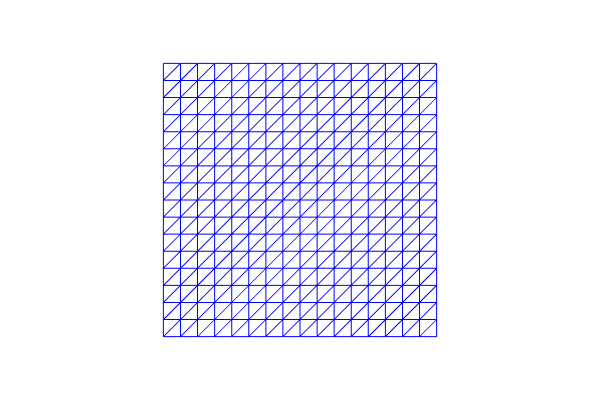
\includegraphics[width=0.48\textwidth]{mesh16.png}
  \end{center}
  \vspace{-20pt}
\end{wrapfigure}
\text{}
\\ \\ Computational domain $\Omega = [0,1]^2$ \\
Inflow Condition \hspace{2mm} $P_{in} = 1$ \\
Outflow Condition \hspace{2mm} $P_{out} = 0$ \\
$\nu = 1/8$ \\ \\ \\ \\ \\ \\ \\
For the coupled solver, our goal is to approximate the fully analytical steady-state flow in 2D.
In the case for the fracstep solver, we will try to imitate the calculations from  (Logg, 2012),
where the numerical calculations are compared to the analytical axial velocity v(1, 0.5) at time $T = 0.5$ shown as.
\begin{align*}
u_x(1, 0.5, t) = 1 - \sum_{N=1,3,..}^{\infty} \frac{32}{\pi^3n^3}
e^{-\frac{\pi^2 n^2}{8}}(-1)^\frac{(n-1)}{2} \\
u_x(1, 0.5, 0.5) \approx 0.44321183655681595
\end{align*}

\newpage
\subsection*{Imlementing 3D pipe}
Computational domain $\Omega = [0,1]^2$ \\ \\ \\
Inflow Condition \hspace{2mm} $P_{in} = 1$ \\ \\ \\
Outflow Condition \hspace{2mm} $P_{out} = 0$ \\ \\

\begin{figure}[h!]
    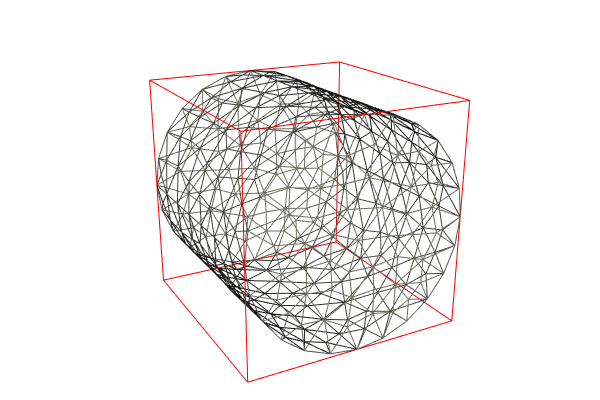
\includegraphics[scale=0.5]{tube.png}
  \caption{A gull}
\end{figure}
For the 3D case aswell, we have the analytical solution for the fully steady-state flow. Here we will
for both coupled and fracstep measure the error for the steady-state case.

\newpage
\section*{Results}
\subsection*{Imlementing 2D pipe}

\end{document}
